% Options for packages loaded elsewhere
\PassOptionsToPackage{unicode}{hyperref}
\PassOptionsToPackage{hyphens}{url}
%
\documentclass[
]{article}
\usepackage{amsmath,amssymb}
\usepackage{lmodern}
\usepackage{ifxetex,ifluatex}
\ifnum 0\ifxetex 1\fi\ifluatex 1\fi=0 % if pdftex
  \usepackage[T1]{fontenc}
  \usepackage[utf8]{inputenc}
  \usepackage{textcomp} % provide euro and other symbols
\else % if luatex or xetex
  \usepackage{unicode-math}
  \defaultfontfeatures{Scale=MatchLowercase}
  \defaultfontfeatures[\rmfamily]{Ligatures=TeX,Scale=1}
\fi
% Use upquote if available, for straight quotes in verbatim environments
\IfFileExists{upquote.sty}{\usepackage{upquote}}{}
\IfFileExists{microtype.sty}{% use microtype if available
  \usepackage[]{microtype}
  \UseMicrotypeSet[protrusion]{basicmath} % disable protrusion for tt fonts
}{}
\makeatletter
\@ifundefined{KOMAClassName}{% if non-KOMA class
  \IfFileExists{parskip.sty}{%
    \usepackage{parskip}
  }{% else
    \setlength{\parindent}{0pt}
    \setlength{\parskip}{6pt plus 2pt minus 1pt}}
}{% if KOMA class
  \KOMAoptions{parskip=half}}
\makeatother
\usepackage{xcolor}
\IfFileExists{xurl.sty}{\usepackage{xurl}}{} % add URL line breaks if available
\IfFileExists{bookmark.sty}{\usepackage{bookmark}}{\usepackage{hyperref}}
\hypersetup{
  pdftitle={M3T2\_FirstContact},
  pdfauthor={Ale F. Benages},
  hidelinks,
  pdfcreator={LaTeX via pandoc}}
\urlstyle{same} % disable monospaced font for URLs
\usepackage[margin=1in]{geometry}
\usepackage{color}
\usepackage{fancyvrb}
\newcommand{\VerbBar}{|}
\newcommand{\VERB}{\Verb[commandchars=\\\{\}]}
\DefineVerbatimEnvironment{Highlighting}{Verbatim}{commandchars=\\\{\}}
% Add ',fontsize=\small' for more characters per line
\usepackage{framed}
\definecolor{shadecolor}{RGB}{248,248,248}
\newenvironment{Shaded}{\begin{snugshade}}{\end{snugshade}}
\newcommand{\AlertTok}[1]{\textcolor[rgb]{0.94,0.16,0.16}{#1}}
\newcommand{\AnnotationTok}[1]{\textcolor[rgb]{0.56,0.35,0.01}{\textbf{\textit{#1}}}}
\newcommand{\AttributeTok}[1]{\textcolor[rgb]{0.77,0.63,0.00}{#1}}
\newcommand{\BaseNTok}[1]{\textcolor[rgb]{0.00,0.00,0.81}{#1}}
\newcommand{\BuiltInTok}[1]{#1}
\newcommand{\CharTok}[1]{\textcolor[rgb]{0.31,0.60,0.02}{#1}}
\newcommand{\CommentTok}[1]{\textcolor[rgb]{0.56,0.35,0.01}{\textit{#1}}}
\newcommand{\CommentVarTok}[1]{\textcolor[rgb]{0.56,0.35,0.01}{\textbf{\textit{#1}}}}
\newcommand{\ConstantTok}[1]{\textcolor[rgb]{0.00,0.00,0.00}{#1}}
\newcommand{\ControlFlowTok}[1]{\textcolor[rgb]{0.13,0.29,0.53}{\textbf{#1}}}
\newcommand{\DataTypeTok}[1]{\textcolor[rgb]{0.13,0.29,0.53}{#1}}
\newcommand{\DecValTok}[1]{\textcolor[rgb]{0.00,0.00,0.81}{#1}}
\newcommand{\DocumentationTok}[1]{\textcolor[rgb]{0.56,0.35,0.01}{\textbf{\textit{#1}}}}
\newcommand{\ErrorTok}[1]{\textcolor[rgb]{0.64,0.00,0.00}{\textbf{#1}}}
\newcommand{\ExtensionTok}[1]{#1}
\newcommand{\FloatTok}[1]{\textcolor[rgb]{0.00,0.00,0.81}{#1}}
\newcommand{\FunctionTok}[1]{\textcolor[rgb]{0.00,0.00,0.00}{#1}}
\newcommand{\ImportTok}[1]{#1}
\newcommand{\InformationTok}[1]{\textcolor[rgb]{0.56,0.35,0.01}{\textbf{\textit{#1}}}}
\newcommand{\KeywordTok}[1]{\textcolor[rgb]{0.13,0.29,0.53}{\textbf{#1}}}
\newcommand{\NormalTok}[1]{#1}
\newcommand{\OperatorTok}[1]{\textcolor[rgb]{0.81,0.36,0.00}{\textbf{#1}}}
\newcommand{\OtherTok}[1]{\textcolor[rgb]{0.56,0.35,0.01}{#1}}
\newcommand{\PreprocessorTok}[1]{\textcolor[rgb]{0.56,0.35,0.01}{\textit{#1}}}
\newcommand{\RegionMarkerTok}[1]{#1}
\newcommand{\SpecialCharTok}[1]{\textcolor[rgb]{0.00,0.00,0.00}{#1}}
\newcommand{\SpecialStringTok}[1]{\textcolor[rgb]{0.31,0.60,0.02}{#1}}
\newcommand{\StringTok}[1]{\textcolor[rgb]{0.31,0.60,0.02}{#1}}
\newcommand{\VariableTok}[1]{\textcolor[rgb]{0.00,0.00,0.00}{#1}}
\newcommand{\VerbatimStringTok}[1]{\textcolor[rgb]{0.31,0.60,0.02}{#1}}
\newcommand{\WarningTok}[1]{\textcolor[rgb]{0.56,0.35,0.01}{\textbf{\textit{#1}}}}
\usepackage{longtable,booktabs,array}
\usepackage{calc} % for calculating minipage widths
% Correct order of tables after \paragraph or \subparagraph
\usepackage{etoolbox}
\makeatletter
\patchcmd\longtable{\par}{\if@noskipsec\mbox{}\fi\par}{}{}
\makeatother
% Allow footnotes in longtable head/foot
\IfFileExists{footnotehyper.sty}{\usepackage{footnotehyper}}{\usepackage{footnote}}
\makesavenoteenv{longtable}
\usepackage{graphicx}
\makeatletter
\def\maxwidth{\ifdim\Gin@nat@width>\linewidth\linewidth\else\Gin@nat@width\fi}
\def\maxheight{\ifdim\Gin@nat@height>\textheight\textheight\else\Gin@nat@height\fi}
\makeatother
% Scale images if necessary, so that they will not overflow the page
% margins by default, and it is still possible to overwrite the defaults
% using explicit options in \includegraphics[width, height, ...]{}
\setkeys{Gin}{width=\maxwidth,height=\maxheight,keepaspectratio}
% Set default figure placement to htbp
\makeatletter
\def\fps@figure{htbp}
\makeatother
\setlength{\emergencystretch}{3em} % prevent overfull lines
\providecommand{\tightlist}{%
  \setlength{\itemsep}{0pt}\setlength{\parskip}{0pt}}
\setcounter{secnumdepth}{-\maxdimen} % remove section numbering
\ifluatex
  \usepackage{selnolig}  % disable illegal ligatures
\fi

\title{M3T2\_FirstContact}
\author{Ale F. Benages}
\date{3/30/2021}

\begin{document}
\maketitle

\hypertarget{library}{%
\section{Library}\label{library}}

\begin{Shaded}
\begin{Highlighting}[]
\FunctionTok{library}\NormalTok{(caret, ggplot2)}
\end{Highlighting}
\end{Shaded}

\begin{verbatim}
## Loading required package: lattice
\end{verbatim}

\begin{verbatim}
## Loading required package: ggplot2
\end{verbatim}

\begin{Shaded}
\begin{Highlighting}[]
\FunctionTok{library}\NormalTok{(ggridges)}
\FunctionTok{library}\NormalTok{(plyr)}
\FunctionTok{library}\NormalTok{(skimr) }\CommentTok{\# to get a fast overview of all the variables. Fast\&Dirty EDA}
\CommentTok{\#library(tictoc)}
\FunctionTok{library}\NormalTok{(mlbench)}
\FunctionTok{library}\NormalTok{(gbm)}
\end{Highlighting}
\end{Shaded}

\begin{verbatim}
## Loaded gbm 2.1.8
\end{verbatim}

\begin{Shaded}
\begin{Highlighting}[]
\FunctionTok{library}\NormalTok{(C50)}
\FunctionTok{set.seed}\NormalTok{(}\DecValTok{9982}\NormalTok{)}
\end{Highlighting}
\end{Shaded}

\hypertarget{load-csv}{%
\section{Load CSV}\label{load-csv}}

\begin{Shaded}
\begin{Highlighting}[]
\NormalTok{path\_to\_file }\OtherTok{\textless{}{-}} \StringTok{"//home/ale/Dropbox/UBIQUM/3.DAwithR/Task2:Classification.in.R/SurveyData/CompleteResponses.csv"}

\NormalTok{ComResp }\OtherTok{\textless{}{-}} \FunctionTok{read.csv}\NormalTok{(path\_to\_file)}

\FunctionTok{str}\NormalTok{(ComResp) }\CommentTok{\# with srt() we can see the structure of the dataframe}
\end{Highlighting}
\end{Shaded}

\begin{verbatim}
## 'data.frame':    9898 obs. of  7 variables:
##  $ salary : num  119807 106880 78021 63690 50874 ...
##  $ age    : int  45 63 23 51 20 56 24 62 29 41 ...
##  $ elevel : int  0 1 0 3 3 3 4 3 4 1 ...
##  $ car    : int  14 11 15 6 14 14 8 3 17 5 ...
##  $ zipcode: int  4 6 2 5 4 3 5 0 0 4 ...
##  $ credit : num  442038 45007 48795 40889 352951 ...
##  $ brand  : int  0 1 0 1 0 1 1 1 0 1 ...
\end{verbatim}

\begin{Shaded}
\begin{Highlighting}[]
\CommentTok{\# head(ComResp) \# with head we get a similar output but with the classic dataframe structure}
\end{Highlighting}
\end{Shaded}

\hypertarget{eda}{%
\section{EDA}\label{eda}}

\textbf{Numerical Variables}\\
* Salary\\
* Age\\
* Credit \textbf{Ordinal Categorical Variables}\\
* elevel \textbf{Nominal Categorical Variables}\\
* Zipcode\\
* Car\\
* Brand

\hypertarget{datatypes}{%
\subsection{Datatypes}\label{datatypes}}

Datatypes from the categorical (ordinal or nominal) variables are
incorrect: \textbf{elevel, car, zipcode and brand} datatypes should be
changed to factor.

\begin{Shaded}
\begin{Highlighting}[]
\CommentTok{\# change the datatype to factor }
\NormalTok{ComResp[, }\StringTok{\textquotesingle{}elevel\textquotesingle{}}\NormalTok{] }\OtherTok{\textless{}{-}} \FunctionTok{as.factor}\NormalTok{(ComResp[, }\StringTok{\textquotesingle{}elevel\textquotesingle{}}\NormalTok{])}
\NormalTok{ComResp[, }\StringTok{\textquotesingle{}car\textquotesingle{}}\NormalTok{] }\OtherTok{\textless{}{-}} \FunctionTok{as.factor}\NormalTok{(ComResp[, }\StringTok{\textquotesingle{}car\textquotesingle{}}\NormalTok{])}
\NormalTok{ComResp[, }\StringTok{\textquotesingle{}zipcode\textquotesingle{}}\NormalTok{] }\OtherTok{\textless{}{-}} \FunctionTok{as.factor}\NormalTok{(ComResp[, }\StringTok{\textquotesingle{}zipcode\textquotesingle{}}\NormalTok{])}
\NormalTok{ComResp[, }\StringTok{\textquotesingle{}brand\textquotesingle{}}\NormalTok{] }\OtherTok{\textless{}{-}} \FunctionTok{as.factor}\NormalTok{(ComResp[, }\StringTok{\textquotesingle{}brand\textquotesingle{}}\NormalTok{])}

\FunctionTok{str}\NormalTok{(ComResp)}
\end{Highlighting}
\end{Shaded}

\begin{verbatim}
## 'data.frame':    9898 obs. of  7 variables:
##  $ salary : num  119807 106880 78021 63690 50874 ...
##  $ age    : int  45 63 23 51 20 56 24 62 29 41 ...
##  $ elevel : Factor w/ 5 levels "0","1","2","3",..: 1 2 1 4 4 4 5 4 5 2 ...
##  $ car    : Factor w/ 20 levels "1","2","3","4",..: 14 11 15 6 14 14 8 3 17 5 ...
##  $ zipcode: Factor w/ 9 levels "0","1","2","3",..: 5 7 3 6 5 4 6 1 1 5 ...
##  $ credit : num  442038 45007 48795 40889 352951 ...
##  $ brand  : Factor w/ 2 levels "0","1": 1 2 1 2 1 2 2 2 1 2 ...
\end{verbatim}

\hypertarget{add-labels}{%
\subsubsection{add labels}\label{add-labels}}

also we can add the corresponding labels to each categorical variable

\begin{Shaded}
\begin{Highlighting}[]
\CommentTok{\# list of labels of elevel}
\NormalTok{ed\_level\_labels }\OtherTok{=} \FunctionTok{c}\NormalTok{(}\StringTok{"Less than High School Degree"}\NormalTok{, }\StringTok{"High School Degree"}\NormalTok{, }\StringTok{"Some College"}\NormalTok{,}\StringTok{"4{-}Year College Degree"}\NormalTok{,}
             \StringTok{"Master\textquotesingle{}s, Doctoral or Professional Degree"}\NormalTok{)}
\CommentTok{\# create a new column \textquotesingle{}elevelLabeled\textquotesingle{}, copy of elevel with values remaped}
\NormalTok{ComResp}\SpecialCharTok{$}\NormalTok{elevelLabeled }\OtherTok{\textless{}{-}} \FunctionTok{mapvalues}\NormalTok{(ComResp}\SpecialCharTok{$}\NormalTok{elevel, }\AttributeTok{from=}\FunctionTok{c}\NormalTok{(}\DecValTok{0}\SpecialCharTok{:}\DecValTok{4}\NormalTok{), }\AttributeTok{to=}\NormalTok{ed\_level\_labels)}

\NormalTok{cars\_labels }\OtherTok{=} \FunctionTok{c}\NormalTok{(}\StringTok{"BMW"}\NormalTok{, }\StringTok{"Buick"}\NormalTok{, }\StringTok{"Cadillac"}\NormalTok{, }\StringTok{"Chevrolet"}\NormalTok{, }\StringTok{"Chrysler"}\NormalTok{, }\StringTok{"Dodge"}\NormalTok{, }\StringTok{"Ford"}\NormalTok{, }\StringTok{"Honda"}\NormalTok{, }\StringTok{"Hyundai"}\NormalTok{, }\StringTok{"Jeep"}\NormalTok{, }\StringTok{"Kia"}\NormalTok{, }\StringTok{"Lincoln"}\NormalTok{, }\StringTok{"Mazda"}\NormalTok{, }\StringTok{"Mercedes Benz"}\NormalTok{, }\StringTok{"Mitsubishi"}\NormalTok{, }\StringTok{"Nissan"}\NormalTok{, }\StringTok{"Ram"}\NormalTok{, }\StringTok{"Subaru"}\NormalTok{, }\StringTok{"Toyota"}\NormalTok{, }\StringTok{"None of the above"}\NormalTok{)}
\NormalTok{ComResp}\SpecialCharTok{$}\NormalTok{carLabeled }\OtherTok{\textless{}{-}} \FunctionTok{mapvalues}\NormalTok{(ComResp}\SpecialCharTok{$}\NormalTok{car, }\AttributeTok{from=}\FunctionTok{c}\NormalTok{(}\DecValTok{0}\SpecialCharTok{:}\DecValTok{19}\NormalTok{), }\AttributeTok{to=}\NormalTok{cars\_labels)}
\end{Highlighting}
\end{Shaded}

\begin{verbatim}
## The following `from` values were not present in `x`: 0
\end{verbatim}

\begin{Shaded}
\begin{Highlighting}[]
\NormalTok{zipcode\_labels }\OtherTok{=} \FunctionTok{c}\NormalTok{(}\StringTok{"New England"}\NormalTok{, }\StringTok{"Mid{-}Atlantic"}\NormalTok{, }\StringTok{"East North Central"}\NormalTok{, }\StringTok{"West North Central"}\NormalTok{, }\StringTok{"South Atlantic"}\NormalTok{, }\StringTok{"East South Central"}\NormalTok{, }\StringTok{"West South Central"}\NormalTok{, }\StringTok{"Mountain"}\NormalTok{, }\StringTok{"Pacific"}\NormalTok{)}
\NormalTok{ComResp}\SpecialCharTok{$}\NormalTok{zipcodeLabeled }\OtherTok{\textless{}{-}} \FunctionTok{mapvalues}\NormalTok{(ComResp}\SpecialCharTok{$}\NormalTok{zipcode, }\AttributeTok{from=}\FunctionTok{c}\NormalTok{(}\DecValTok{0}\SpecialCharTok{:}\DecValTok{8}\NormalTok{), }\AttributeTok{to=}\NormalTok{zipcode\_labels)}

\NormalTok{brands\_labels }\OtherTok{=} \FunctionTok{c}\NormalTok{(}\StringTok{"Acer"}\NormalTok{, }\StringTok{"Sony"}\NormalTok{)}
\NormalTok{ComResp}\SpecialCharTok{$}\NormalTok{brandLabeled }\OtherTok{\textless{}{-}} \FunctionTok{mapvalues}\NormalTok{(ComResp}\SpecialCharTok{$}\NormalTok{brand, }\AttributeTok{from=}\FunctionTok{c}\NormalTok{(}\DecValTok{0}\SpecialCharTok{:}\DecValTok{1}\NormalTok{), }\AttributeTok{to=}\NormalTok{brands\_labels)}
\end{Highlighting}
\end{Shaded}

the Skim function gives us a great overview of the dataset

\begin{Shaded}
\begin{Highlighting}[]
\FunctionTok{skim}\NormalTok{(ComResp)}
\end{Highlighting}
\end{Shaded}

\begin{longtable}[]{@{}ll@{}}
\caption{Data summary}\tabularnewline
\toprule
& \\
\midrule
\endfirsthead
\toprule
& \\
\midrule
\endhead
Name & ComResp \\
Number of rows & 9898 \\
Number of columns & 11 \\
\_\_\_\_\_\_\_\_\_\_\_\_\_\_\_\_\_\_\_\_\_\_\_ & \\
Column type frequency: & \\
factor & 8 \\
numeric & 3 \\
\_\_\_\_\_\_\_\_\_\_\_\_\_\_\_\_\_\_\_\_\_\_\_\_ & \\
Group variables & None \\
\bottomrule
\end{longtable}

\textbf{Variable type: factor}

\begin{longtable}[]{@{}lrrlrl@{}}
\toprule
skim\_variable & n\_missing & complete\_rate & ordered & n\_unique &
top\_counts \\
\midrule
\endhead
elevel & 0 & 1 & FALSE & 5 & 0: 2052, 2: 1983, 4: 1968, 1: 1948 \\
car & 0 & 1 & FALSE & 20 & 15: 542, 18: 524, 8: 511, 2: 509 \\
zipcode & 0 & 1 & FALSE & 9 & 6: 1155, 8: 1135, 2: 1112, 5: 1108 \\
brand & 0 & 1 & FALSE & 2 & 1: 6154, 0: 3744 \\
elevelLabeled & 0 & 1 & FALSE & 5 & Les: 2052, Som: 1983, Mas: 1968,
Hig: 1948 \\
carLabeled & 0 & 1 & FALSE & 20 & Nis: 542, Toy: 524, Hyu: 511, Cad:
509 \\
zipcodeLabeled & 0 & 1 & FALSE & 9 & Wes: 1155, Pac: 1135, Eas: 1112,
Eas: 1108 \\
brandLabeled & 0 & 1 & FALSE & 2 & Son: 6154, Ace: 3744 \\
\bottomrule
\end{longtable}

\textbf{Variable type: numeric}

\begin{longtable}[]{@{}lrrrrrrrrrl@{}}
\toprule
skim\_variable & n\_missing & complete\_rate & mean & sd & p0 & p25 &
p50 & p75 & p100 & hist \\
\midrule
\endhead
salary & 0 & 1 & 84870.86 & 37712.34 & 20000 & 52082.11 & 84949.74 &
117162.0 & 150000 & ▇▇▇▇▇ \\
age & 0 & 1 & 49.78 & 17.60 & 20 & 35.00 & 50.00 & 65.0 & 80 & ▇▇▇▇▇ \\
credit & 0 & 1 & 249175.97 & 145211.57 & 0 & 120806.81 & 250607.15 &
374639.7 & 500000 & ▇▇▇▇▇ \\
\bottomrule
\end{longtable}

\hypertarget{missing-values-and-na}{%
\subsection{Missing values and NA ?}\label{missing-values-and-na}}

\begin{itemize}
\tightlist
\item
  No missing values
\end{itemize}

\hypertarget{plots-of-each-variables.}{%
\subsection{Plots of each variables.}\label{plots-of-each-variables.}}

\hypertarget{salary}{%
\subsubsection{1. Salary}\label{salary}}

Survey Questions and Response Key\\
1) What is your yearly salary, not including bonuses?. Respondents enter
numeric value

\begin{itemize}
\tightlist
\item
  \textbf{This is a numerical variable. }
\end{itemize}

\begin{Shaded}
\begin{Highlighting}[]
\FunctionTok{summary}\NormalTok{(ComResp}\SpecialCharTok{$}\NormalTok{salary)}
\end{Highlighting}
\end{Shaded}

\begin{verbatim}
##    Min. 1st Qu.  Median    Mean 3rd Qu.    Max. 
##   20000   52082   84950   84871  117162  150000
\end{verbatim}

\begin{Shaded}
\begin{Highlighting}[]
\FunctionTok{ggplot}\NormalTok{( ComResp, }\FunctionTok{aes}\NormalTok{(}\AttributeTok{x=}\NormalTok{salary)) }\SpecialCharTok{+} \FunctionTok{theme\_bw}\NormalTok{()}\SpecialCharTok{+}
  \FunctionTok{geom\_histogram}\NormalTok{(}\AttributeTok{color =} \StringTok{\textquotesingle{}black\textquotesingle{}}\NormalTok{, }\AttributeTok{fill =} \StringTok{\textquotesingle{}\#FF6620\textquotesingle{}}\NormalTok{, }\AttributeTok{binwidth =} \DecValTok{10000}\NormalTok{)}\SpecialCharTok{+}
  \FunctionTok{labs}\NormalTok{(}\AttributeTok{title =} \StringTok{"Salary Distribution"}\NormalTok{, }\AttributeTok{x=}\StringTok{"Salary"}\NormalTok{) }\SpecialCharTok{+} 
  \FunctionTok{geom\_vline}\NormalTok{(}\FunctionTok{aes}\NormalTok{(}\AttributeTok{xintercept=}\FunctionTok{mean}\NormalTok{(salary)), }\AttributeTok{color=}\StringTok{"blue"}\NormalTok{, }\AttributeTok{linetype=}\StringTok{"dashed"}\NormalTok{, }\AttributeTok{size=}\DecValTok{1}\NormalTok{)  }\CommentTok{\# adds the mean}
\end{Highlighting}
\end{Shaded}

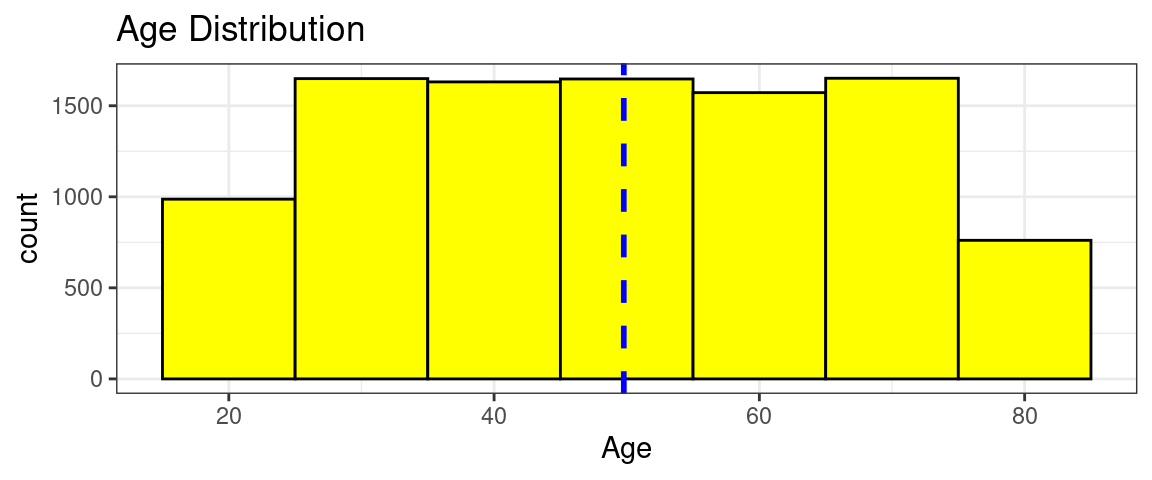
\includegraphics{M3T2_FirstContact_2_files/figure-latex/unnamed-chunk-7-1.pdf}

\hypertarget{age}{%
\subsubsection{2. Age}\label{age}}

Survey Questions and Response Key\\
2) What is your age?. Respondents enter numeric value

\begin{itemize}
\tightlist
\item
  ** This is a Numerical Variable**
\end{itemize}

\begin{Shaded}
\begin{Highlighting}[]
\FunctionTok{summary}\NormalTok{(ComResp}\SpecialCharTok{$}\NormalTok{age)}
\end{Highlighting}
\end{Shaded}

\begin{verbatim}
##    Min. 1st Qu.  Median    Mean 3rd Qu.    Max. 
##   20.00   35.00   50.00   49.78   65.00   80.00
\end{verbatim}

\begin{Shaded}
\begin{Highlighting}[]
\FunctionTok{ggplot}\NormalTok{( ComResp, }\FunctionTok{aes}\NormalTok{(}\AttributeTok{x=}\NormalTok{age)) }\SpecialCharTok{+} \FunctionTok{theme\_bw}\NormalTok{()}\SpecialCharTok{+}
  \FunctionTok{geom\_histogram}\NormalTok{(}\AttributeTok{color =} \StringTok{\textquotesingle{}black\textquotesingle{}}\NormalTok{, }\AttributeTok{fill =} \StringTok{\textquotesingle{}yellow\textquotesingle{}}\NormalTok{, }\AttributeTok{binwidth =} \DecValTok{10}\NormalTok{)}\SpecialCharTok{+}
  \FunctionTok{labs}\NormalTok{(}\AttributeTok{title =} \StringTok{"Age Distribution"}\NormalTok{, }\AttributeTok{x=}\StringTok{"Age"}\NormalTok{) }\SpecialCharTok{+}
  \FunctionTok{geom\_vline}\NormalTok{(}\FunctionTok{aes}\NormalTok{(}\AttributeTok{xintercept=}\FunctionTok{mean}\NormalTok{(age)), }\AttributeTok{color=}\StringTok{"blue"}\NormalTok{, }\AttributeTok{linetype=}\StringTok{"dashed"}\NormalTok{, }\AttributeTok{size=}\DecValTok{1}\NormalTok{)  }\CommentTok{\# adds the mean}
\end{Highlighting}
\end{Shaded}

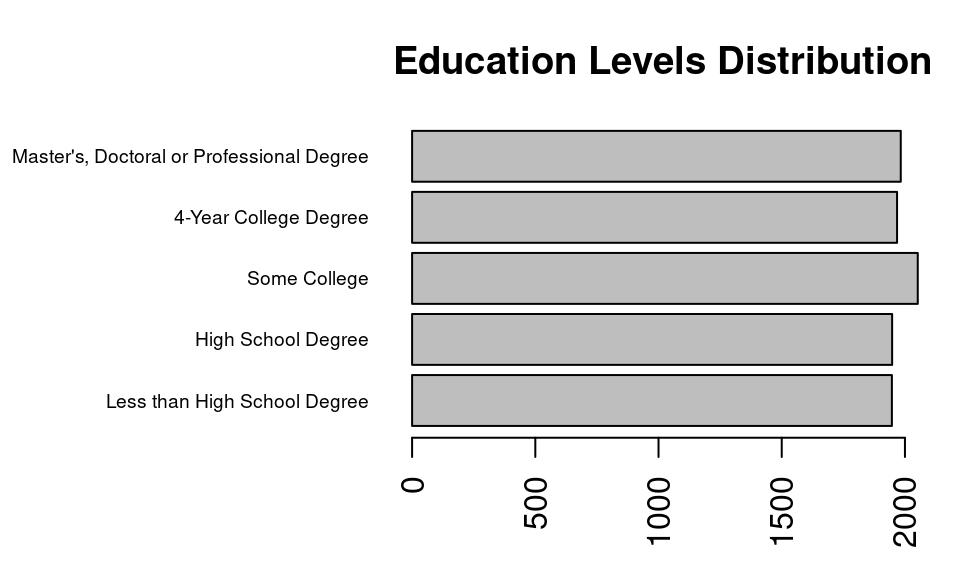
\includegraphics{M3T2_FirstContact_2_files/figure-latex/unnamed-chunk-9-1.pdf}
\textgreater{} in general the customers have 30 to 70 years old.

\hypertarget{elevel---education-level}{%
\subsubsection{3. elevel - Education
Level}\label{elevel---education-level}}

\begin{enumerate}
\def\labelenumi{\arabic{enumi})}
\setcounter{enumi}{2}
\tightlist
\item
  What is the highest level of education you have obtained?. Respondents
  select from the following 5 choices:\\
  Value : Description\\
  0 : Less than High School Degree\\
  1 : High School Degree\\
  2 : Some College\\
  3 : 4-Year College Degree\\
  4 : Master's, Doctoral or Professional Degree
\end{enumerate}

\begin{itemize}
\tightlist
\item
  \textbf{This is a categorical ordinal variable}
\end{itemize}

\begin{Shaded}
\begin{Highlighting}[]
\CommentTok{\# print the head just to verify everything is correct}
\FunctionTok{head}\NormalTok{(ComResp)}
\end{Highlighting}
\end{Shaded}

\begin{verbatim}
##      salary age elevel car zipcode    credit brand                elevelLabeled
## 1 119806.54  45      0  14       4 442037.71     0 Less than High School Degree
## 2 106880.48  63      1  11       6  45007.18     1           High School Degree
## 3  78020.75  23      0  15       2  48795.32     0 Less than High School Degree
## 4  63689.94  51      3   6       5  40888.88     1        4-Year College Degree
## 5  50873.62  20      3  14       4 352951.50     0        4-Year College Degree
## 6 130812.74  56      3  14       3 135943.02     1        4-Year College Degree
##   carLabeled     zipcodeLabeled brandLabeled
## 1 Mitsubishi     South Atlantic         Acer
## 2    Lincoln West South Central         Sony
## 3     Nissan East North Central         Acer
## 4       Ford East South Central         Sony
## 5 Mitsubishi     South Atlantic         Acer
## 6 Mitsubishi West North Central         Sony
\end{verbatim}

\begin{Shaded}
\begin{Highlighting}[]
\CommentTok{\# magins of the plot}
\CommentTok{\# mar: A numerical vector of the form c(bottom, left, top, right) which gives }
\CommentTok{\# the number of lines of margin to be specified on the four sides of the plot. }
\CommentTok{\# The default is c(5, 4, 4, 2) + 0.1.}
\FunctionTok{par}\NormalTok{(}\AttributeTok{mar=}\FunctionTok{c}\NormalTok{(}\FloatTok{3.5}\NormalTok{,}\FloatTok{10.5}\NormalTok{,}\DecValTok{3}\NormalTok{,}\DecValTok{1}\NormalTok{)}\SpecialCharTok{+}\FloatTok{0.1}\NormalTok{)}

\NormalTok{counts }\OtherTok{\textless{}{-}} \FunctionTok{table}\NormalTok{(ComResp}\SpecialCharTok{$}\NormalTok{elevelLabeled)}

\CommentTok{\# finally a Simple Horizontal Bar Plot with Added Labels}
\FunctionTok{barplot}\NormalTok{(counts, }\AttributeTok{main=}\StringTok{"Education Levels Distribution"}\NormalTok{, }\AttributeTok{horiz=}\ConstantTok{TRUE}\NormalTok{, }\AttributeTok{names.arg=}\NormalTok{ed\_level\_labels, }\AttributeTok{cex.names=}\FloatTok{0.6}\NormalTok{, }\AttributeTok{las=}\DecValTok{2}\NormalTok{)}
\end{Highlighting}
\end{Shaded}

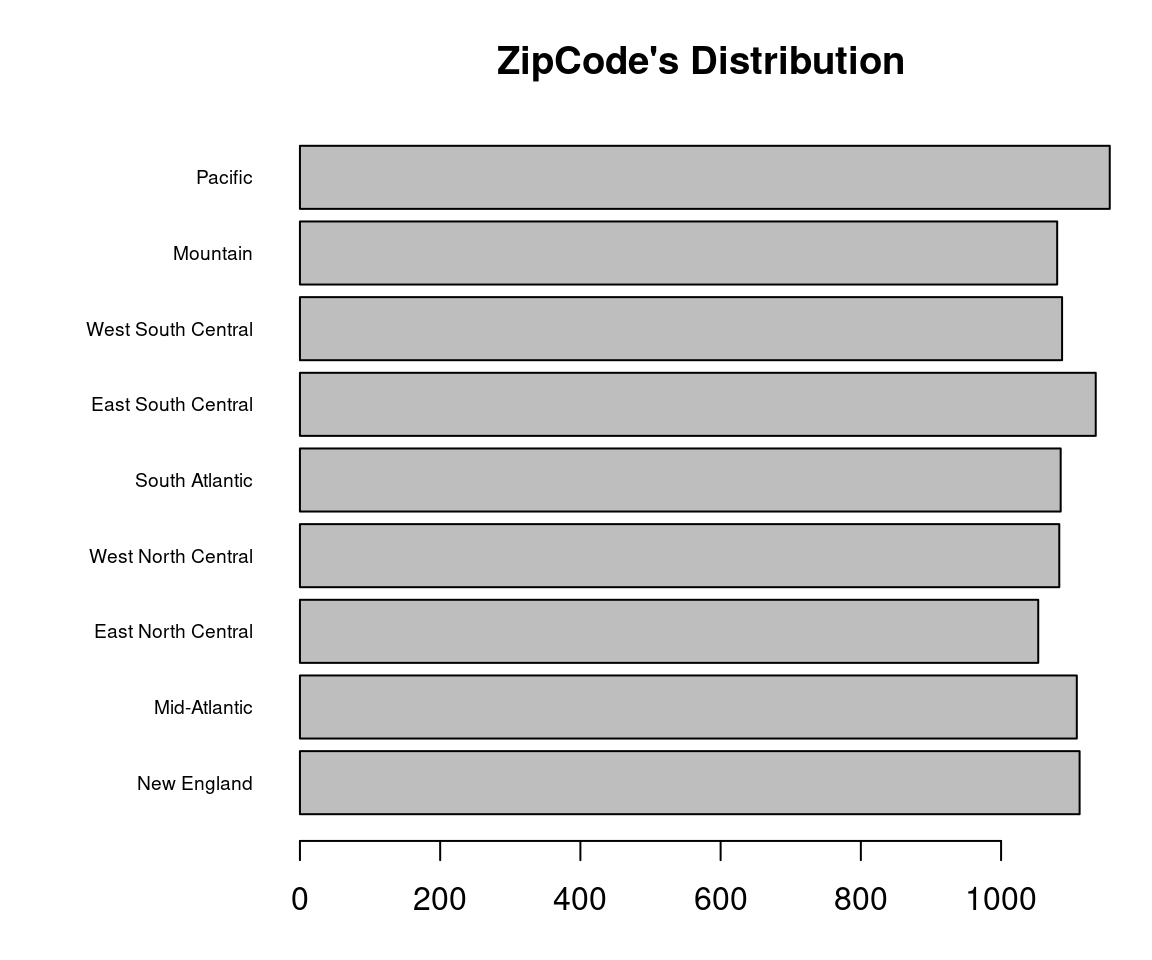
\includegraphics{M3T2_FirstContact_2_files/figure-latex/unnamed-chunk-11-1.pdf}
\textgreater{} In general the education level of customers is very
homogeneous.

\hypertarget{car}{%
\subsubsection{4. Car}\label{car}}

\begin{enumerate}
\def\labelenumi{\arabic{enumi})}
\setcounter{enumi}{3}
\tightlist
\item
  What is the make of your primary car?. Respondents select from the
  following 20 choices: Value : Description 1 : BMW\\
  2 : Buick\\
  3 : Cadillac\\
  4 : Chevrolet\\
  5 : Chrysler\\
  6 : Dodge\\
  7 : Ford\\
  8 : Honda\\
  9 : Hyundai\\
  10 : Jeep\\
  11 : Kia\\
  12 : Lincoln\\
  13 : Mazda\\
  14 : Mercedes Benz\\
  15 : Mitsubishi\\
  16 : Nissan\\
  17 : Ram\\
  18 : Subaru\\
  19 : Toyota\\
  20 : None of the above
\end{enumerate}

\begin{itemize}
\tightlist
\item
  \textbf{this is a Nominal categorical variable}
\end{itemize}

\begin{Shaded}
\begin{Highlighting}[]
\CommentTok{\# Simple Horizontal Bar Plot with Added Labels}
\FunctionTok{par}\NormalTok{(}\AttributeTok{mar=}\FunctionTok{c}\NormalTok{(}\DecValTok{3}\NormalTok{,}\FloatTok{7.5}\NormalTok{,}\DecValTok{3}\NormalTok{,}\DecValTok{1}\NormalTok{)}\SpecialCharTok{+}\FloatTok{0.1}\NormalTok{)}
\CommentTok{\# mar: A numerical vector of the form c(bottom, left, top, right) which gives }
\CommentTok{\# the number of lines of margin to be specified on the four sides of the plot. }
\CommentTok{\# The default is c(5, 4, 4, 2) + 0.1.}

\NormalTok{Car\_counts }\OtherTok{\textless{}{-}} \FunctionTok{table}\NormalTok{(ComResp}\SpecialCharTok{$}\NormalTok{carLabeled)}

\FunctionTok{barplot}\NormalTok{(Car\_counts, }\AttributeTok{main=}\StringTok{"Car\textquotesingle{}s Brands Distribution"}\NormalTok{, }\AttributeTok{horiz=}\ConstantTok{TRUE}\NormalTok{, }\AttributeTok{names.arg=}\NormalTok{cars\_labels, }\AttributeTok{cex.names=}\FloatTok{0.6}\NormalTok{, }\AttributeTok{las=}\DecValTok{1}\NormalTok{,)}
\end{Highlighting}
\end{Shaded}

\includegraphics{M3T2_FirstContact_2_files/figure-latex/unnamed-chunk-12-1.pdf}

\begin{quote}
There is no preffered car's brand. the chocices are very homogeneous.
\end{quote}

\hypertarget{zipcode}{%
\subsubsection{5. zipcode}\label{zipcode}}

\begin{enumerate}
\def\labelenumi{\arabic{enumi})}
\setcounter{enumi}{4}
\tightlist
\item
  What is your zip code?. Respondents enter zip code, which is captured
  as 1 of the following 9 regions in the U.S.\\
  Value : Region\\
  0 : New England\\
  1 : Mid-Atlantic\\
  2 : East North Central\\
  3 : West North Central\\
  4 : South Atlantic\\
  5 : East South Central\\
  6 : West South Central\\
  7 : Mountain\\
  8 : Pacific
\end{enumerate}

\begin{itemize}
\tightlist
\item
  \textbf{This is a categorical Nominal variable}
\end{itemize}

\begin{Shaded}
\begin{Highlighting}[]
\CommentTok{\# Simple Horizontal Bar Plot with Added Labels}
\FunctionTok{par}\NormalTok{(}\AttributeTok{mar=}\FunctionTok{c}\NormalTok{(}\DecValTok{3}\NormalTok{,}\FloatTok{7.5}\NormalTok{,}\DecValTok{3}\NormalTok{,}\DecValTok{1}\NormalTok{)}\SpecialCharTok{+}\FloatTok{0.1}\NormalTok{)}
\CommentTok{\# mar: A numerical vector of the form c(bottom, left, top, right) which gives }
\CommentTok{\# the number of lines of margin to be specified on the four sides of the plot. }
\CommentTok{\# The default is c(5, 4, 4, 2) + 0.1.}

\NormalTok{zipcode\_counts }\OtherTok{\textless{}{-}} \FunctionTok{table}\NormalTok{(ComResp}\SpecialCharTok{$}\NormalTok{zipcodeLabeled)}

\FunctionTok{barplot}\NormalTok{(zipcode\_counts, }\AttributeTok{main=}\StringTok{"ZipCode\textquotesingle{}s Distribution"}\NormalTok{, }\AttributeTok{horiz=}\ConstantTok{TRUE}\NormalTok{, }\AttributeTok{names.arg=}\NormalTok{zipcode\_labels, }\AttributeTok{cex.names=}\FloatTok{0.6}\NormalTok{, }\AttributeTok{las=}\DecValTok{1}\NormalTok{,)}
\end{Highlighting}
\end{Shaded}

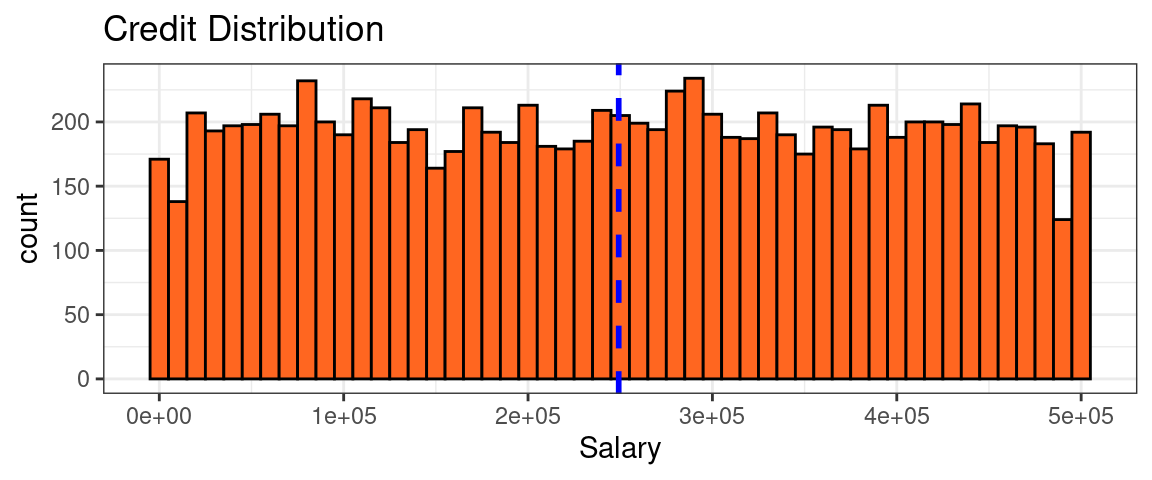
\includegraphics{M3T2_FirstContact_2_files/figure-latex/unnamed-chunk-13-1.pdf}

\hypertarget{credit}{%
\subsubsection{6. Credit}\label{credit}}

\begin{enumerate}
\def\labelenumi{\arabic{enumi})}
\setcounter{enumi}{5}
\tightlist
\item
  What amount of credit is available to you?. Respondents enter numeric
  value.
\end{enumerate}

\begin{itemize}
\tightlist
\item
  \textbf{Quantitative variable}
\end{itemize}

\begin{Shaded}
\begin{Highlighting}[]
\FunctionTok{summary}\NormalTok{(ComResp}\SpecialCharTok{$}\NormalTok{credit)}
\end{Highlighting}
\end{Shaded}

\begin{verbatim}
##    Min. 1st Qu.  Median    Mean 3rd Qu.    Max. 
##       0  120807  250607  249176  374640  500000
\end{verbatim}

\begin{Shaded}
\begin{Highlighting}[]
\FunctionTok{ggplot}\NormalTok{( ComResp, }\FunctionTok{aes}\NormalTok{(}\AttributeTok{x=}\NormalTok{credit)) }\SpecialCharTok{+} \FunctionTok{theme\_bw}\NormalTok{()}\SpecialCharTok{+}
  \FunctionTok{geom\_histogram}\NormalTok{(}\AttributeTok{color =} \StringTok{\textquotesingle{}black\textquotesingle{}}\NormalTok{, }\AttributeTok{fill =} \StringTok{\textquotesingle{}\#FF6620\textquotesingle{}}\NormalTok{, }\AttributeTok{binwidth =} \DecValTok{10000}\NormalTok{)}\SpecialCharTok{+}
  \FunctionTok{labs}\NormalTok{(}\AttributeTok{title =} \StringTok{"Credit Distribution"}\NormalTok{, }\AttributeTok{x=}\StringTok{"Salary"}\NormalTok{) }\SpecialCharTok{+} 
  \FunctionTok{geom\_vline}\NormalTok{(}\FunctionTok{aes}\NormalTok{(}\AttributeTok{xintercept=}\FunctionTok{mean}\NormalTok{(credit)), }\AttributeTok{color=}\StringTok{"blue"}\NormalTok{, }\AttributeTok{linetype=}\StringTok{"dashed"}\NormalTok{, }\AttributeTok{size=}\DecValTok{1}\NormalTok{)  }\CommentTok{\# this line adds the mean}
\end{Highlighting}
\end{Shaded}

\includegraphics{M3T2_FirstContact_2_files/figure-latex/unnamed-chunk-15-1.pdf}

\hypertarget{brand}{%
\subsubsection{7. brand}\label{brand}}

\begin{enumerate}
\def\labelenumi{\arabic{enumi})}
\setcounter{enumi}{6}
\tightlist
\item
  Which brand of computers do you prefer?. Respondents select from the
  following 2 choices:\\
  Value : Description\\
  0 : Acer\\
  1 : Sony
\end{enumerate}

\begin{quote}
this is our \textbf{Target variable.}
\end{quote}

\begin{Shaded}
\begin{Highlighting}[]
\NormalTok{brand\_table }\OtherTok{\textless{}{-}} \FunctionTok{table}\NormalTok{(ComResp}\SpecialCharTok{$}\NormalTok{brand)}

\FunctionTok{barplot}\NormalTok{(brand\_table, }
        \AttributeTok{col =} \FunctionTok{rainbow}\NormalTok{(}\DecValTok{2}\NormalTok{), }
        \AttributeTok{names.arg =} \FunctionTok{c}\NormalTok{(}\StringTok{"Acer"}\NormalTok{, }\StringTok{"Sony"}\NormalTok{))}
\end{Highlighting}
\end{Shaded}

\includegraphics{M3T2_FirstContact_2_files/figure-latex/unnamed-chunk-16-1.pdf}

\hypertarget{normalization}{%
\subsection{Normalization}\label{normalization}}

The formula for a min-max normalization is:
\[(X – min(X))/(max(X) – min(X))\] For each value of a variable, we
simply find how far that value is from the minimum value, then divide by
the range. To implement this in R, we can define a simple function and
then use lapply to apply that function to whichever columns in the
dataset:

\begin{Shaded}
\begin{Highlighting}[]
\CommentTok{\#define Min{-}Max normalization function}
\NormalTok{min\_max\_norm }\OtherTok{\textless{}{-}} \ControlFlowTok{function}\NormalTok{(x) \{ }
\NormalTok{  (x }\SpecialCharTok{{-}} \FunctionTok{min}\NormalTok{(x)) }\SpecialCharTok{/}\NormalTok{ (}\FunctionTok{max}\NormalTok{(x) }\SpecialCharTok{{-}} \FunctionTok{min}\NormalTok{(x))}
\NormalTok{  \}}
\end{Highlighting}
\end{Shaded}

\begin{Shaded}
\begin{Highlighting}[]
\CommentTok{\#apply Min{-}Max normalization to the numerical variables}
\NormalTok{ComResp\_norm }\OtherTok{\textless{}{-}} \FunctionTok{as.data.frame}\NormalTok{(}\FunctionTok{lapply}\NormalTok{(ComResp[}\FunctionTok{c}\NormalTok{(}\StringTok{\textquotesingle{}salary\textquotesingle{}}\NormalTok{,}\StringTok{\textquotesingle{}age\textquotesingle{}}\NormalTok{,}\StringTok{\textquotesingle{}credit\textquotesingle{}}\NormalTok{)], min\_max\_norm))}
\CommentTok{\#print structure}
\FunctionTok{str}\NormalTok{(ComResp\_norm)}
\end{Highlighting}
\end{Shaded}

\begin{verbatim}
## 'data.frame':    9898 obs. of  3 variables:
##  $ salary: num  0.768 0.668 0.446 0.336 0.237 ...
##  $ age   : num  0.417 0.717 0.05 0.517 0 ...
##  $ credit: num  0.8841 0.09 0.0976 0.0818 0.7059 ...
\end{verbatim}

\begin{Shaded}
\begin{Highlighting}[]
\CommentTok{\#summary}
\FunctionTok{summary}\NormalTok{(ComResp\_norm)}
\end{Highlighting}
\end{Shaded}

\begin{verbatim}
##      salary            age             credit      
##  Min.   :0.0000   Min.   :0.0000   Min.   :0.0000  
##  1st Qu.:0.2468   1st Qu.:0.2500   1st Qu.:0.2416  
##  Median :0.4996   Median :0.5000   Median :0.5012  
##  Mean   :0.4990   Mean   :0.4963   Mean   :0.4984  
##  3rd Qu.:0.7474   3rd Qu.:0.7500   3rd Qu.:0.7493  
##  Max.   :1.0000   Max.   :1.0000   Max.   :1.0000
\end{verbatim}

The result looks great, all the numerical variables from 0 to 1, and
also they are very symmetric. 1Q is close to 0.25, Mean
\textasciitilde{} 0.5 and 3Q \textasciitilde{} 0.75.\\
But notice that all the rest of the variables were dropped out. They
must be added manually.

\begin{Shaded}
\begin{Highlighting}[]
\NormalTok{ComResp\_norm}\SpecialCharTok{$}\NormalTok{elevel }\OtherTok{\textless{}{-}}\NormalTok{ ComResp}\SpecialCharTok{$}\NormalTok{elevel }
\NormalTok{ComResp\_norm}\SpecialCharTok{$}\NormalTok{car }\OtherTok{\textless{}{-}}\NormalTok{ ComResp}\SpecialCharTok{$}\NormalTok{car}
\NormalTok{ComResp\_norm}\SpecialCharTok{$}\NormalTok{zipcode }\OtherTok{\textless{}{-}}\NormalTok{ ComResp}\SpecialCharTok{$}\NormalTok{zipcode}
\NormalTok{ComResp\_norm}\SpecialCharTok{$}\NormalTok{brand }\OtherTok{\textless{}{-}}\NormalTok{ ComResp}\SpecialCharTok{$}\NormalTok{brand}

\CommentTok{\#ComResp\_norm$elevelLabeled \textless{}{-} ComResp$elevelLabeled }
\CommentTok{\#ComResp\_norm$carLabeled \textless{}{-} ComResp$carLabeled}
\CommentTok{\#ComResp\_norm$zipcodeLabeled \textless{}{-} ComResp$zipcodeLabeled}
\CommentTok{\#ComResp\_norm$brandLabeled \textless{}{-} ComResp$brandLabeled}

\FunctionTok{str}\NormalTok{(ComResp\_norm)}
\end{Highlighting}
\end{Shaded}

\begin{verbatim}
## 'data.frame':    9898 obs. of  7 variables:
##  $ salary : num  0.768 0.668 0.446 0.336 0.237 ...
##  $ age    : num  0.417 0.717 0.05 0.517 0 ...
##  $ credit : num  0.8841 0.09 0.0976 0.0818 0.7059 ...
##  $ elevel : Factor w/ 5 levels "0","1","2","3",..: 1 2 1 4 4 4 5 4 5 2 ...
##  $ car    : Factor w/ 20 levels "1","2","3","4",..: 14 11 15 6 14 14 8 3 17 5 ...
##  $ zipcode: Factor w/ 9 levels "0","1","2","3",..: 5 7 3 6 5 4 6 1 1 5 ...
##  $ brand  : Factor w/ 2 levels "0","1": 1 2 1 2 1 2 2 2 1 2 ...
\end{verbatim}

\hypertarget{train-the-models}{%
\section{Train the Models}\label{train-the-models}}

\hypertarget{traintest-split}{%
\subsection{Train/Test Split}\label{traintest-split}}

\begin{Shaded}
\begin{Highlighting}[]
\CommentTok{\# define an 75\%/25\% train/test split of the dataset}
\NormalTok{inTraining }\OtherTok{\textless{}{-}}\NormalTok{ caret}\SpecialCharTok{::}\FunctionTok{createDataPartition}\NormalTok{(ComResp\_norm}\SpecialCharTok{$}\NormalTok{brand, }\AttributeTok{p =}\NormalTok{ .}\DecValTok{75}\NormalTok{, }\AttributeTok{list =} \ConstantTok{FALSE}\NormalTok{)}
\NormalTok{training }\OtherTok{\textless{}{-}}\NormalTok{ ComResp\_norm[inTraining,]}
\NormalTok{testing }\OtherTok{\textless{}{-}}\NormalTok{ ComResp\_norm[}\SpecialCharTok{{-}}\NormalTok{inTraining,]}
\end{Highlighting}
\end{Shaded}

\hypertarget{models}{%
\subsection{Models}\label{models}}

\begin{quote}
Models training commented, to avoid execution.
\end{quote}

\hypertarget{load-the-models}{%
\subsection{Load the Models}\label{load-the-models}}

as I avoided the execution of the models, but previously saved them, I
load them from them memory

\begin{Shaded}
\begin{Highlighting}[]
\NormalTok{gbmFit1 }\OtherTok{\textless{}{-}} \FunctionTok{readRDS}\NormalTok{(}\StringTok{"./Models/gbmFit1.rds"}\NormalTok{)}
\NormalTok{gbmFit2 }\OtherTok{\textless{}{-}} \FunctionTok{readRDS}\NormalTok{ (}\StringTok{\textquotesingle{}./Models/gbmFit2.rds\textquotesingle{}}\NormalTok{)}
\NormalTok{rfFit1 }\OtherTok{\textless{}{-}} \FunctionTok{readRDS}\NormalTok{ (}\StringTok{\textquotesingle{}./Models/rfmFit1.rds\textquotesingle{}}\NormalTok{)}
\NormalTok{rfFit2 }\OtherTok{\textless{}{-}} \FunctionTok{readRDS}\NormalTok{ (}\StringTok{\textquotesingle{}./Models/rfmFit2.rds\textquotesingle{}}\NormalTok{)}
\NormalTok{rfFit3 }\OtherTok{\textless{}{-}} \FunctionTok{readRDS}\NormalTok{ (}\StringTok{\textquotesingle{}./Models/rfmFit3.rds\textquotesingle{}}\NormalTok{)}
\NormalTok{c50Fit }\OtherTok{\textless{}{-}} \FunctionTok{readRDS}\NormalTok{ (}\StringTok{\textquotesingle{}./Models/c50Fit.rds\textquotesingle{}}\NormalTok{)}
\end{Highlighting}
\end{Shaded}

\hypertarget{predictions-on-the-complete-survey---ground-truth}{%
\subsection{Predictions on the Complete Survey - (Ground
Truth)}\label{predictions-on-the-complete-survey---ground-truth}}

\begin{Shaded}
\begin{Highlighting}[]
\FunctionTok{print}\NormalTok{(}\StringTok{\textquotesingle{}GBM1\textquotesingle{}}\NormalTok{)}
\end{Highlighting}
\end{Shaded}

\begin{verbatim}
## [1] "GBM1"
\end{verbatim}

\begin{Shaded}
\begin{Highlighting}[]
\NormalTok{brand\_prediction\_GBM }\OtherTok{\textless{}{-}} \FunctionTok{predict}\NormalTok{(gbmFit1, testing)   }\CommentTok{\# does the prediction predict(model, testData)}
\FunctionTok{postResample}\NormalTok{(brand\_prediction\_GBM, testing}\SpecialCharTok{$}\NormalTok{brand)  }\CommentTok{\# After making the predictions using the }
\end{Highlighting}
\end{Shaded}

\begin{verbatim}
##  Accuracy     Kappa 
## 0.9264349 0.8452281
\end{verbatim}

\begin{Shaded}
\begin{Highlighting}[]
\FunctionTok{print}\NormalTok{(}\StringTok{\textquotesingle{}GBM2\textquotesingle{}}\NormalTok{)}
\end{Highlighting}
\end{Shaded}

\begin{verbatim}
## [1] "GBM2"
\end{verbatim}

\begin{Shaded}
\begin{Highlighting}[]
\NormalTok{brand\_prediction\_GBM }\OtherTok{\textless{}{-}} \FunctionTok{predict}\NormalTok{(gbmFit2, testing)   }\CommentTok{\# does the prediction predict(model, testData)}
\FunctionTok{postResample}\NormalTok{(brand\_prediction\_GBM, testing}\SpecialCharTok{$}\NormalTok{brand)  }\CommentTok{\# After making the predictions using the }
\end{Highlighting}
\end{Shaded}

\begin{verbatim}
##  Accuracy     Kappa 
## 0.9288601 0.8505161
\end{verbatim}

\begin{Shaded}
\begin{Highlighting}[]
\CommentTok{\#brand\_prediction\_GBM \textless{}{-} predict(gbmFit2, testing\_reduced)   \# does the prediction predict(model, testData)}
\CommentTok{\#postResample(brand\_prediction\_GBM, testing\_reduced$brandLabeled)  \# After making the predictions using the test set use postResample() to assess the metrics of the new predictions compared to the Ground Truth }

\FunctionTok{print}\NormalTok{(}\StringTok{\textquotesingle{}RF1\textquotesingle{}}\NormalTok{)}
\end{Highlighting}
\end{Shaded}

\begin{verbatim}
## [1] "RF1"
\end{verbatim}

\begin{Shaded}
\begin{Highlighting}[]
\NormalTok{brand\_prediction\_RF1 }\OtherTok{\textless{}{-}} \FunctionTok{predict}\NormalTok{(rfFit1, testing)}
\FunctionTok{postResample}\NormalTok{(brand\_prediction\_RF1, testing}\SpecialCharTok{$}\NormalTok{brand)}
\end{Highlighting}
\end{Shaded}

\begin{verbatim}
##  Accuracy     Kappa 
## 0.9248181 0.8410371
\end{verbatim}

\begin{Shaded}
\begin{Highlighting}[]
\CommentTok{\#brand\_prediction\_RF1 \textless{}{-} predict(rfFit1, testing\_reduced)}
\CommentTok{\#postResample(brand\_prediction\_RF1, testing\_reduced$brandLabeled)}

\FunctionTok{print}\NormalTok{(}\StringTok{\textquotesingle{}RF2\textquotesingle{}}\NormalTok{)}
\end{Highlighting}
\end{Shaded}

\begin{verbatim}
## [1] "RF2"
\end{verbatim}

\begin{Shaded}
\begin{Highlighting}[]
\NormalTok{brand\_prediction\_RF2 }\OtherTok{\textless{}{-}} \FunctionTok{predict}\NormalTok{(rfFit2, testing)}
\FunctionTok{postResample}\NormalTok{(brand\_prediction\_RF2, testing}\SpecialCharTok{$}\NormalTok{brand)}
\end{Highlighting}
\end{Shaded}

\begin{verbatim}
##  Accuracy     Kappa 
## 0.9296686 0.8509828
\end{verbatim}

\begin{Shaded}
\begin{Highlighting}[]
\CommentTok{\#brand\_prediction\_RF2 \textless{}{-} predict(rfFit2, testing\_reduced)}
\CommentTok{\#postResample(brand\_prediction\_RF2, testing\_reduced$brandLabeled)}


\FunctionTok{print}\NormalTok{(}\StringTok{\textquotesingle{}RF3\textquotesingle{}}\NormalTok{)}
\end{Highlighting}
\end{Shaded}

\begin{verbatim}
## [1] "RF3"
\end{verbatim}

\begin{Shaded}
\begin{Highlighting}[]
\NormalTok{brand\_prediction\_RF3 }\OtherTok{\textless{}{-}} \FunctionTok{predict}\NormalTok{(rfFit3, testing)}
\FunctionTok{postResample}\NormalTok{(brand\_prediction\_RF3, testing}\SpecialCharTok{$}\NormalTok{brand)}
\end{Highlighting}
\end{Shaded}

\begin{verbatim}
##  Accuracy     Kappa 
## 0.9292643 0.8504070
\end{verbatim}

\begin{Shaded}
\begin{Highlighting}[]
\CommentTok{\#brand\_prediction\_RF3 \textless{}{-} predict(rfFit3, testing\_reduced)}
\CommentTok{\#postResample(brand\_prediction\_RF3, testing\_reduced$brandLabeled)}

\FunctionTok{print}\NormalTok{(}\StringTok{\textquotesingle{}C5.0\textquotesingle{}}\NormalTok{)}
\end{Highlighting}
\end{Shaded}

\begin{verbatim}
## [1] "C5.0"
\end{verbatim}

\begin{Shaded}
\begin{Highlighting}[]
\NormalTok{brand\_prediction\_c50 }\OtherTok{\textless{}{-}} \FunctionTok{predict}\NormalTok{(c50Fit, testing)}
\FunctionTok{postResample}\NormalTok{(brand\_prediction\_c50, testing}\SpecialCharTok{$}\NormalTok{brand)}
\end{Highlighting}
\end{Shaded}

\begin{verbatim}
##  Accuracy     Kappa 
## 0.8439774 0.6681770
\end{verbatim}

\begin{Shaded}
\begin{Highlighting}[]
\CommentTok{\#brand\_prediction\_c50 \textless{}{-} predict(c50Fit, testing\_reduced)}
\CommentTok{\#postResample(brand\_prediction\_c50, testing\_reduced$brandLabeled)}
\end{Highlighting}
\end{Shaded}

\hypertarget{select-a-model}{%
\subsubsection{Select a model}\label{select-a-model}}

Based on the results of the predictions, the bests models are:

\begin{quote}
``RF2'' \textgreater{} rfFit2 \textgreater{} Accuracy: 0.9296686\\
``RF3'' \textgreater{} rfFit3 \textgreater{} Accuracy: 0.9292643\\
``GBM2'' \textgreater{} gbmFit2 \textgreater{} Accuracy: 0.9288601
\end{quote}

\hypertarget{remove-redundant-data}{%
\subsubsection{Remove redundant data}\label{remove-redundant-data}}

Based on the result of the varImp(rfFit2) the most important features
are:\\
* Salary * Age * credit

So we can remove the rest of the variables to improve performance and
reduce computational costs.

\begin{Shaded}
\begin{Highlighting}[]
\NormalTok{ComResp\_norm\_reduced }\OtherTok{\textless{}{-}}\NormalTok{ ComResp\_norm }\CommentTok{\#creates a copy of the DF}
\NormalTok{ComResp\_norm\_reduced}\SpecialCharTok{$}\NormalTok{elevel }\OtherTok{\textless{}{-}} \ConstantTok{NULL}  \CommentTok{\#removes the elevel variable}
\NormalTok{ComResp\_norm\_reduced}\SpecialCharTok{$}\NormalTok{car }\OtherTok{\textless{}{-}} \ConstantTok{NULL}
\NormalTok{ComResp\_norm\_reduced}\SpecialCharTok{$}\NormalTok{zipcode }\OtherTok{\textless{}{-}} \ConstantTok{NULL}
\NormalTok{ComResp\_norm\_reduced}\SpecialCharTok{$}\NormalTok{brand }\OtherTok{\textless{}{-}} \ConstantTok{NULL}  \CommentTok{\#as we have the brandLabeled, this is useless}
\end{Highlighting}
\end{Shaded}

In the training I forgot to add the labels to the brand, and it's
useful\ldots{}

\begin{Shaded}
\begin{Highlighting}[]
\NormalTok{brands\_labels }\OtherTok{=} \FunctionTok{c}\NormalTok{(}\StringTok{"Acer"}\NormalTok{, }\StringTok{"Sony"}\NormalTok{)}
\NormalTok{ComResp\_norm\_reduced}\SpecialCharTok{$}\NormalTok{brandLabeled }\OtherTok{\textless{}{-}} \FunctionTok{mapvalues}\NormalTok{(ComResp\_norm}\SpecialCharTok{$}\NormalTok{brand, }\AttributeTok{from=}\FunctionTok{c}\NormalTok{(}\DecValTok{0}\SpecialCharTok{:}\DecValTok{1}\NormalTok{), }\AttributeTok{to=}\NormalTok{brands\_labels)}
\end{Highlighting}
\end{Shaded}

\begin{Shaded}
\begin{Highlighting}[]
\FunctionTok{str}\NormalTok{(ComResp\_norm\_reduced)}
\end{Highlighting}
\end{Shaded}

\begin{verbatim}
## 'data.frame':    9898 obs. of  4 variables:
##  $ salary      : num  0.768 0.668 0.446 0.336 0.237 ...
##  $ age         : num  0.417 0.717 0.05 0.517 0 ...
##  $ credit      : num  0.8841 0.09 0.0976 0.0818 0.7059 ...
##  $ brandLabeled: Factor w/ 2 levels "Acer","Sony": 1 2 1 2 1 2 2 2 1 2 ...
\end{verbatim}

just to check if everything still nice\ldots{} train again the RF2 with
the reduced dataset

\begin{Shaded}
\begin{Highlighting}[]
\CommentTok{\# train/test split of the dataset}
\NormalTok{inTraining\_reduced }\OtherTok{\textless{}{-}} \FunctionTok{createDataPartition}\NormalTok{(ComResp\_norm\_reduced}\SpecialCharTok{$}\NormalTok{brandLabeled, }\AttributeTok{p =}\NormalTok{ .}\DecValTok{75}\NormalTok{, }\AttributeTok{list =} \ConstantTok{FALSE}\NormalTok{)}
\NormalTok{training\_reduced }\OtherTok{\textless{}{-}}\NormalTok{ ComResp\_norm\_reduced[inTraining\_reduced,]}
\NormalTok{testing\_reduced }\OtherTok{\textless{}{-}}\NormalTok{ ComResp\_norm\_reduced[}\SpecialCharTok{{-}}\NormalTok{inTraining\_reduced,]}
\end{Highlighting}
\end{Shaded}

Commented this part of the code to avoid execution. But the model is
saved in memory.

\hypertarget{load-the-models-1}{%
\subsection{Load the Models}\label{load-the-models-1}}

as I avoided the execution of the models, but previously saved them, I
load them from them memory

\begin{Shaded}
\begin{Highlighting}[]
\NormalTok{rfFit2\_reduced }\OtherTok{\textless{}{-}} \FunctionTok{readRDS}\NormalTok{(}\StringTok{"./Models/rfFit2\_reduced.rds"}\NormalTok{)}
\end{Highlighting}
\end{Shaded}

\begin{Shaded}
\begin{Highlighting}[]
\NormalTok{predictions\_reduced }\OtherTok{\textless{}{-}} \FunctionTok{predict}\NormalTok{(rfFit2\_reduced, testing\_reduced)}
\FunctionTok{summary}\NormalTok{(predictions\_reduced)}
\end{Highlighting}
\end{Shaded}

\begin{verbatim}
## Acer Sony 
##  942 1532
\end{verbatim}

\begin{Shaded}
\begin{Highlighting}[]
\FunctionTok{confusionMatrix}\NormalTok{(predictions\_reduced, testing\_reduced}\SpecialCharTok{$}\NormalTok{brandLabeled)}
\end{Highlighting}
\end{Shaded}

\begin{verbatim}
## Confusion Matrix and Statistics
## 
##           Reference
## Prediction Acer Sony
##       Acer  919   23
##       Sony   17 1515
##                                          
##                Accuracy : 0.9838         
##                  95% CI : (0.978, 0.9884)
##     No Information Rate : 0.6217         
##     P-Value [Acc > NIR] : <2e-16         
##                                          
##                   Kappa : 0.9657         
##                                          
##  Mcnemar's Test P-Value : 0.4292         
##                                          
##             Sensitivity : 0.9818         
##             Specificity : 0.9850         
##          Pos Pred Value : 0.9756         
##          Neg Pred Value : 0.9889         
##              Prevalence : 0.3783         
##          Detection Rate : 0.3715         
##    Detection Prevalence : 0.3808         
##       Balanced Accuracy : 0.9834         
##                                          
##        'Positive' Class : Acer           
## 
\end{verbatim}

\hypertarget{incomlpete-survey}{%
\section{Incomlpete Survey}\label{incomlpete-survey}}

\hypertarget{load-csv---incomplete}{%
\subsection{Load CSV - Incomplete}\label{load-csv---incomplete}}

\begin{Shaded}
\begin{Highlighting}[]
\NormalTok{path\_to\_file }\OtherTok{\textless{}{-}} \StringTok{"//home/ale/Dropbox/UBIQUM/3.DAwithR/Task2:Classification.in.R/SurveyData/SurveyIncomplete.csv"}

\NormalTok{IncompleteResp }\OtherTok{\textless{}{-}} \FunctionTok{read.csv}\NormalTok{(path\_to\_file)}

\FunctionTok{str}\NormalTok{(IncompleteResp) }\CommentTok{\# with srt() we can see the structure of the dataframe}
\end{Highlighting}
\end{Shaded}

\begin{verbatim}
## 'data.frame':    5000 obs. of  7 variables:
##  $ salary : num  150000 82524 115647 141443 149211 ...
##  $ age    : int  76 51 34 22 56 26 64 50 26 46 ...
##  $ elevel : int  1 1 0 3 0 4 3 3 2 3 ...
##  $ car    : int  3 8 10 18 5 12 1 9 3 18 ...
##  $ zipcode: int  3 3 2 2 3 1 2 0 4 6 ...
##  $ credit : num  377980 141658 360980 282736 215667 ...
##  $ brand  : int  1 0 1 1 1 1 1 1 1 0 ...
\end{verbatim}

\hypertarget{drop-unnecesary-data}{%
\subsection{Drop Unnecesary data}\label{drop-unnecesary-data}}

the first thing I will do is remove the unnecessary data. Two main
groups:\\
- from feature selection \textgreater\textgreater{} remove(elevel, car,
zipcode, and credit)\\
- and i will remove also the brand column. It should be empty, but
actually has inconsistent data: some `ones' at the beginin and then full
of `zeros'. Will remove it and the main task of this part will be
guessing them.

\begin{Shaded}
\begin{Highlighting}[]
\NormalTok{IncompleteResp\_reduced }\OtherTok{\textless{}{-}}\NormalTok{ IncompleteResp }\CommentTok{\#creates a copy of the DF}
\NormalTok{IncompleteResp\_reduced}\SpecialCharTok{$}\NormalTok{elevel }\OtherTok{\textless{}{-}} \ConstantTok{NULL}
\NormalTok{IncompleteResp\_reduced}\SpecialCharTok{$}\NormalTok{car }\OtherTok{\textless{}{-}} \ConstantTok{NULL}
\NormalTok{IncompleteResp\_reduced}\SpecialCharTok{$}\NormalTok{zipcode }\OtherTok{\textless{}{-}} \ConstantTok{NULL}
\NormalTok{IncompleteResp\_reduced}\SpecialCharTok{$}\NormalTok{brand }\OtherTok{\textless{}{-}} \ConstantTok{NULL} 

\FunctionTok{str}\NormalTok{(IncompleteResp\_reduced) }\CommentTok{\#take a look to the reduced DF}
\end{Highlighting}
\end{Shaded}

\begin{verbatim}
## 'data.frame':    5000 obs. of  3 variables:
##  $ salary: num  150000 82524 115647 141443 149211 ...
##  $ age   : int  76 51 34 22 56 26 64 50 26 46 ...
##  $ credit: num  377980 141658 360980 282736 215667 ...
\end{verbatim}

\hypertarget{eda-1}{%
\subsection{EDA}\label{eda-1}}

\begin{Shaded}
\begin{Highlighting}[]
\FunctionTok{skim}\NormalTok{(IncompleteResp\_reduced)}
\end{Highlighting}
\end{Shaded}

\begin{longtable}[]{@{}ll@{}}
\caption{Data summary}\tabularnewline
\toprule
& \\
\midrule
\endfirsthead
\toprule
& \\
\midrule
\endhead
Name & IncompleteResp\_reduced \\
Number of rows & 5000 \\
Number of columns & 3 \\
\_\_\_\_\_\_\_\_\_\_\_\_\_\_\_\_\_\_\_\_\_\_\_ & \\
Column type frequency: & \\
numeric & 3 \\
\_\_\_\_\_\_\_\_\_\_\_\_\_\_\_\_\_\_\_\_\_\_\_\_ & \\
Group variables & None \\
\bottomrule
\end{longtable}

\textbf{Variable type: numeric}

\begin{longtable}[]{@{}lrrrrrrrrrl@{}}
\toprule
skim\_variable & n\_missing & complete\_rate & mean & sd & p0 & p25 &
p50 & p75 & p100 & hist \\
\midrule
\endhead
salary & 0 & 1 & 85793.81 & 37800.01 & 20000 & 52589.96 & 86220.72 &
118535.2 & 150000 & ▇▇▇▇▇ \\
age & 0 & 1 & 49.94 & 17.67 & 20 & 35.00 & 50.00 & 65.0 & 80 & ▇▇▇▇▇ \\
credit & 0 & 1 & 249546.21 & 145859.26 & 0 & 122310.71 & 250973.69 &
375652.7 & 500000 & ▇▇▇▇▇ \\
\bottomrule
\end{longtable}

\begin{itemize}
\item
  no missing values.
\item
  from a fast and simple comparative of the Quantiles ans mean, Salady
  and Age from the complete and incomplete survey are very similar!.
  \textgreater\textgreater{} would be nice to plot two histograms
  overlayed, comparing the distributions.
\end{itemize}

\hypertarget{normalization-1}{%
\subsubsection{Normalization}\label{normalization-1}}

\begin{Shaded}
\begin{Highlighting}[]
\CommentTok{\#apply Min{-}Max normalization to the numerical variables}
\NormalTok{IncompleteResp\_reduced\_norm }\OtherTok{\textless{}{-}} \FunctionTok{as.data.frame}\NormalTok{(}\FunctionTok{lapply}\NormalTok{(IncompleteResp\_reduced[}\FunctionTok{c}\NormalTok{(}\StringTok{\textquotesingle{}salary\textquotesingle{}}\NormalTok{,}\StringTok{\textquotesingle{}age\textquotesingle{}}\NormalTok{,}\StringTok{\textquotesingle{}credit\textquotesingle{}}\NormalTok{)], min\_max\_norm))}
\FunctionTok{str}\NormalTok{(IncompleteResp\_reduced\_norm)}
\end{Highlighting}
\end{Shaded}

\begin{verbatim}
## 'data.frame':    5000 obs. of  3 variables:
##  $ salary: num  1 0.481 0.736 0.934 0.994 ...
##  $ age   : num  0.9333 0.5167 0.2333 0.0333 0.6 ...
##  $ credit: num  0.756 0.283 0.722 0.565 0.431 ...
\end{verbatim}

\hypertarget{traintest-split.}{%
\subsection{Train/Test Split.}\label{traintest-split.}}

I this case I want to guess the brand choice, out target variable, from
the \emph{Incomplete Survey}. I don't have this information, so it's
useless to do the train/test split. In this case the entire set is used
to make predictions.

\hypertarget{load-the-model}{%
\subsection{Load the model}\label{load-the-model}}

will load the saved copy of the model: \textbf{RF2\_reduced}

\begin{Shaded}
\begin{Highlighting}[]
\NormalTok{super\_model }\OtherTok{\textless{}{-}} \FunctionTok{readRDS}\NormalTok{(}\StringTok{"./Models/rfFit2\_reduced.rds"}\NormalTok{)}
\FunctionTok{print}\NormalTok{(super\_model)}
\end{Highlighting}
\end{Shaded}

\begin{verbatim}
## Random Forest 
## 
## 7424 samples
##    3 predictor
##    2 classes: 'Acer', 'Sony' 
## 
## No pre-processing
## Resampling: Cross-Validated (10 fold, repeated 5 times) 
## Summary of sample sizes: 6682, 6682, 6682, 6682, 6681, 6681, ... 
## Resampling results across tuning parameters:
## 
##   mtry  Accuracy   Kappa    
##   1     0.9206092  0.8314534
##   2     0.9167307  0.8231428
## 
## Accuracy was used to select the optimal model using the largest value.
## The final value used for the model was mtry = 1.
\end{verbatim}

\hypertarget{guessing}{%
\subsection{Guessing!}\label{guessing}}

I'm using the RF2 to guess the brand choice of the incomplete survey.

\begin{Shaded}
\begin{Highlighting}[]
\NormalTok{guess }\OtherTok{\textless{}{-}} \FunctionTok{predict}\NormalTok{(super\_model, IncompleteResp\_reduced\_norm)}
\FunctionTok{summary}\NormalTok{(guess)}
\end{Highlighting}
\end{Shaded}

\begin{verbatim}
## Acer Sony 
## 1903 3097
\end{verbatim}

\begin{Shaded}
\begin{Highlighting}[]
\FunctionTok{plot}\NormalTok{(guess)}
\end{Highlighting}
\end{Shaded}

\includegraphics{M3T2_FirstContact_2_files/figure-latex/unnamed-chunk-34-1.pdf}

\hypertarget{analysis}{%
\section{Analysis}\label{analysis}}

\hypertarget{samples-analisis}{%
\subsection{Samples Analisis}\label{samples-analisis}}

A sample is just a part of a population. It is important to compare the
distribution of samples in the survey.

\hypertarget{salary-1}{%
\subsubsection{Salary}\label{salary-1}}

\begin{Shaded}
\begin{Highlighting}[]
\FunctionTok{options}\NormalTok{(}\AttributeTok{scipen =} \DecValTok{999}\NormalTok{) }\CommentTok{\# removes scientific notation}
\FunctionTok{ggplot}\NormalTok{(ComResp, }\FunctionTok{aes}\NormalTok{(}\AttributeTok{x=}\NormalTok{salary)) }\SpecialCharTok{+} \FunctionTok{geom\_density}\NormalTok{(}\AttributeTok{fill=}\StringTok{"\#69b3a2"}\NormalTok{, }\AttributeTok{color=}\StringTok{"red"}\NormalTok{) }\SpecialCharTok{+} \FunctionTok{ggtitle}\NormalTok{(}\StringTok{"Salary {-} Complete survey"}\NormalTok{)}
\end{Highlighting}
\end{Shaded}

\includegraphics{M3T2_FirstContact_2_files/figure-latex/unnamed-chunk-35-1.pdf}

\begin{Shaded}
\begin{Highlighting}[]
\FunctionTok{ggplot}\NormalTok{(IncompleteResp, }\FunctionTok{aes}\NormalTok{(}\AttributeTok{x=}\NormalTok{salary)) }\SpecialCharTok{+} \FunctionTok{geom\_density}\NormalTok{(}\AttributeTok{fill=}\StringTok{"\#69b3a2"}\NormalTok{, }\AttributeTok{color=}\StringTok{"blue"}\NormalTok{) }\SpecialCharTok{+} \FunctionTok{ggtitle}\NormalTok{(}\StringTok{"Salary {-} Incomplete survey"}\NormalTok{)}
\end{Highlighting}
\end{Shaded}

\includegraphics{M3T2_FirstContact_2_files/figure-latex/unnamed-chunk-35-2.pdf}

\begin{Shaded}
\begin{Highlighting}[]
\FunctionTok{ggplot}\NormalTok{(ComResp, }\FunctionTok{aes}\NormalTok{(}\AttributeTok{x=}\NormalTok{salary)) }\SpecialCharTok{+} \FunctionTok{geom\_boxplot}\NormalTok{(}\AttributeTok{fill=}\StringTok{"\#A19F99"}\NormalTok{, }\AttributeTok{color=}\StringTok{"red"}\NormalTok{)  }\SpecialCharTok{+} \FunctionTok{ggtitle}\NormalTok{(}\StringTok{"Salary {-} Complete survey"}\NormalTok{)}
\end{Highlighting}
\end{Shaded}

\includegraphics{M3T2_FirstContact_2_files/figure-latex/unnamed-chunk-35-3.pdf}

\begin{Shaded}
\begin{Highlighting}[]
\FunctionTok{ggplot}\NormalTok{(IncompleteResp, }\FunctionTok{aes}\NormalTok{(}\AttributeTok{x=}\NormalTok{salary)) }\SpecialCharTok{+} \FunctionTok{geom\_boxplot}\NormalTok{(}\AttributeTok{fill=}\StringTok{"\#A19F99"}\NormalTok{, }\AttributeTok{color=}\StringTok{"blue"}\NormalTok{) }\SpecialCharTok{+} \FunctionTok{ggtitle}\NormalTok{(}\StringTok{"Salary {-} Incomplete survey"}\NormalTok{) }
\end{Highlighting}
\end{Shaded}

\includegraphics{M3T2_FirstContact_2_files/figure-latex/unnamed-chunk-35-4.pdf}

\hypertarget{age-1}{%
\subsubsection{Age}\label{age-1}}

\begin{Shaded}
\begin{Highlighting}[]
\FunctionTok{options}\NormalTok{(}\AttributeTok{scipen =} \DecValTok{999}\NormalTok{) }\CommentTok{\# removes scientific notation}
\FunctionTok{ggplot}\NormalTok{(ComResp, }\FunctionTok{aes}\NormalTok{(}\AttributeTok{x=}\NormalTok{age)) }\SpecialCharTok{+}
    \FunctionTok{geom\_density}\NormalTok{(}\AttributeTok{fill=}\StringTok{"\#69b3a2"}\NormalTok{, }\AttributeTok{color=}\StringTok{"red"}\NormalTok{) }\SpecialCharTok{+} 
  \FunctionTok{ggtitle}\NormalTok{(}\StringTok{"Age {-} Complete survey"}\NormalTok{)}
\end{Highlighting}
\end{Shaded}

\includegraphics{M3T2_FirstContact_2_files/figure-latex/unnamed-chunk-36-1.pdf}

\begin{Shaded}
\begin{Highlighting}[]
\FunctionTok{ggplot}\NormalTok{(IncompleteResp, }\FunctionTok{aes}\NormalTok{(}\AttributeTok{x=}\NormalTok{age)) }\SpecialCharTok{+}
    \FunctionTok{geom\_density}\NormalTok{(}\AttributeTok{fill=}\StringTok{"\#69b3a2"}\NormalTok{, }\AttributeTok{color=}\StringTok{"blue"}\NormalTok{) }\SpecialCharTok{+} 
  \FunctionTok{ggtitle}\NormalTok{(}\StringTok{"Age {-} Incomplete survey"}\NormalTok{)}
\end{Highlighting}
\end{Shaded}

\includegraphics{M3T2_FirstContact_2_files/figure-latex/unnamed-chunk-36-2.pdf}

\begin{Shaded}
\begin{Highlighting}[]
\FunctionTok{ggplot}\NormalTok{(ComResp, }\FunctionTok{aes}\NormalTok{(}\AttributeTok{x=}\NormalTok{age)) }\SpecialCharTok{+} \FunctionTok{geom\_boxplot}\NormalTok{(}\AttributeTok{fill=}\StringTok{"\#56B4E9"}\NormalTok{, }\AttributeTok{color=}\StringTok{"red"}\NormalTok{) }\SpecialCharTok{+} \FunctionTok{ggtitle}\NormalTok{(}\StringTok{"Age {-} Complete survey"}\NormalTok{)}
\end{Highlighting}
\end{Shaded}

\includegraphics{M3T2_FirstContact_2_files/figure-latex/unnamed-chunk-36-3.pdf}

\begin{Shaded}
\begin{Highlighting}[]
\FunctionTok{ggplot}\NormalTok{(IncompleteResp, }\FunctionTok{aes}\NormalTok{(}\AttributeTok{x=}\NormalTok{age)) }\SpecialCharTok{+} \FunctionTok{geom\_boxplot}\NormalTok{(}\AttributeTok{fill=}\StringTok{"\#56B4E9"}\NormalTok{, }\AttributeTok{color=}\StringTok{"Blue"}\NormalTok{)  }\SpecialCharTok{+} \FunctionTok{ggtitle}\NormalTok{(}\StringTok{"Age {-} Incomplete survey"}\NormalTok{)}
\end{Highlighting}
\end{Shaded}

\includegraphics{M3T2_FirstContact_2_files/figure-latex/unnamed-chunk-36-4.pdf}

\hypertarget{credit-1}{%
\subsubsection{Credit}\label{credit-1}}

\begin{Shaded}
\begin{Highlighting}[]
\FunctionTok{options}\NormalTok{(}\AttributeTok{scipen =} \DecValTok{999}\NormalTok{) }\CommentTok{\# removes scientific notation}

\FunctionTok{ggplot}\NormalTok{(ComResp, }\FunctionTok{aes}\NormalTok{(}\AttributeTok{x=}\NormalTok{credit)) }\SpecialCharTok{+}
    \FunctionTok{geom\_density}\NormalTok{(}\AttributeTok{fill=}\StringTok{"\#69b3a2"}\NormalTok{, }\AttributeTok{color=}\StringTok{"red"}\NormalTok{) }\SpecialCharTok{+} 
    \FunctionTok{ggtitle}\NormalTok{(}\StringTok{"Credit {-} Complete survey"}\NormalTok{)}
\end{Highlighting}
\end{Shaded}

\includegraphics{M3T2_FirstContact_2_files/figure-latex/unnamed-chunk-37-1.pdf}

\begin{Shaded}
\begin{Highlighting}[]
\FunctionTok{ggplot}\NormalTok{(IncompleteResp, }\FunctionTok{aes}\NormalTok{(}\AttributeTok{x=}\NormalTok{credit)) }\SpecialCharTok{+}
    \FunctionTok{geom\_density}\NormalTok{(}\AttributeTok{fill=}\StringTok{"\#69b3a2"}\NormalTok{, }\AttributeTok{color=}\StringTok{"blue"}\NormalTok{) }\SpecialCharTok{+} 
  \FunctionTok{ggtitle}\NormalTok{(}\StringTok{"Credit {-} Incomplete survey"}\NormalTok{)}
\end{Highlighting}
\end{Shaded}

\includegraphics{M3T2_FirstContact_2_files/figure-latex/unnamed-chunk-37-2.pdf}

\begin{Shaded}
\begin{Highlighting}[]
\FunctionTok{ggplot}\NormalTok{(ComResp, }\FunctionTok{aes}\NormalTok{(}\AttributeTok{x=}\NormalTok{credit)) }\SpecialCharTok{+} \FunctionTok{geom\_boxplot}\NormalTok{(}\AttributeTok{fill=}\StringTok{"\#E69F00"}\NormalTok{, }\AttributeTok{color=}\StringTok{"red"}\NormalTok{)  }\SpecialCharTok{+} \FunctionTok{ggtitle}\NormalTok{(}\StringTok{"Credit {-} Complete survey"}\NormalTok{)  }
\end{Highlighting}
\end{Shaded}

\includegraphics{M3T2_FirstContact_2_files/figure-latex/unnamed-chunk-37-3.pdf}

\begin{Shaded}
\begin{Highlighting}[]
\FunctionTok{ggplot}\NormalTok{(IncompleteResp, }\FunctionTok{aes}\NormalTok{(}\AttributeTok{x=}\NormalTok{credit)) }\SpecialCharTok{+} \FunctionTok{geom\_boxplot}\NormalTok{(}\AttributeTok{fill=}\StringTok{"\#E69F00"}\NormalTok{, }\AttributeTok{color=}\StringTok{"blue"}\NormalTok{) }\SpecialCharTok{+} \FunctionTok{ggtitle}\NormalTok{(}\StringTok{"Credit {-} Incomplete survey"}\NormalTok{)}
\end{Highlighting}
\end{Shaded}

\includegraphics{M3T2_FirstContact_2_files/figure-latex/unnamed-chunk-37-4.pdf}

\hypertarget{analysis-of-proportions}{%
\subsection{Analysis of Proportions}\label{analysis-of-proportions}}

\begin{itemize}
\tightlist
\item
  Guessed Proportion of Acer/Sony
\end{itemize}

\begin{Shaded}
\begin{Highlighting}[]
\NormalTok{coso }\OtherTok{\textless{}{-}} \FunctionTok{summary}\NormalTok{(guess)}
\NormalTok{guess\_DF }\OtherTok{\textless{}{-}} \FunctionTok{as.data.frame}\NormalTok{(coso) }
\CommentTok{\#head(guess\_DF)}

\CommentTok{\# calculates the proportion of sony }
\NormalTok{proportion\_guessed\_sony }\OtherTok{=}\NormalTok{ guess\_DF[}\DecValTok{1}\NormalTok{,}\DecValTok{1}\NormalTok{]}\SpecialCharTok{/}\NormalTok{guess\_DF[}\DecValTok{2}\NormalTok{,}\DecValTok{1}\NormalTok{]}
\CommentTok{\#proportion\_guessed\_sony}

\CommentTok{\# acer = 1 {-} sony}
\NormalTok{proportion\_guessed\_acer }\OtherTok{=} \DecValTok{1}\SpecialCharTok{{-}}\NormalTok{ proportion\_guessed\_sony}
\CommentTok{\#proportion\_guessed\_acer}

\CommentTok{\# add those values to a DF}
\NormalTok{vec }\OtherTok{\textless{}{-}} \FunctionTok{c}\NormalTok{(proportion\_guessed\_acer, proportion\_guessed\_sony) }
\NormalTok{guess\_DF}\SpecialCharTok{$}\NormalTok{prop\_guess }\OtherTok{\textless{}{-}}\NormalTok{ vec}


\NormalTok{guess\_DF}\SpecialCharTok{$}\NormalTok{coso }\OtherTok{\textless{}{-}} \ConstantTok{NULL}  \CommentTok{\# elimino esta column temporal que no uso. }
\FunctionTok{head}\NormalTok{(guess\_DF)}
\end{Highlighting}
\end{Shaded}

\begin{verbatim}
##      prop_guess
## Acer  0.3855344
## Sony  0.6144656
\end{verbatim}

\begin{itemize}
\tightlist
\item
  True Proportion of Acer/Sony
\end{itemize}

\begin{Shaded}
\begin{Highlighting}[]
\NormalTok{coso2 }\OtherTok{\textless{}{-}} \FunctionTok{summary}\NormalTok{(ComResp}\SpecialCharTok{$}\NormalTok{brandLabeled)}
\NormalTok{trueProportion\_DF }\OtherTok{\textless{}{-}} \FunctionTok{as.data.frame}\NormalTok{(coso2) }
\CommentTok{\#head(trueProportion\_DF)}
\NormalTok{proportion\_true\_sony }\OtherTok{=}\NormalTok{ trueProportion\_DF[}\DecValTok{1}\NormalTok{,}\DecValTok{1}\NormalTok{]}\SpecialCharTok{/}\NormalTok{trueProportion\_DF[}\DecValTok{2}\NormalTok{,}\DecValTok{1}\NormalTok{]}
\CommentTok{\#proportion\_true\_sony}
\NormalTok{proportion\_true\_acer }\OtherTok{=} \DecValTok{1}\SpecialCharTok{{-}}\NormalTok{proportion\_true\_sony}
\CommentTok{\#proportion\_true\_acer}

\CommentTok{\# add those values to a DF}
\NormalTok{vec }\OtherTok{\textless{}{-}} \FunctionTok{c}\NormalTok{(proportion\_true\_acer, proportion\_true\_sony) }
\NormalTok{guess\_DF}\SpecialCharTok{$}\NormalTok{prop\_true }\OtherTok{\textless{}{-}}\NormalTok{ vec}

\NormalTok{allValues }\OtherTok{\textless{}{-}} \FunctionTok{c}\NormalTok{(proportion\_true\_acer, proportion\_guessed\_acer, proportion\_true\_sony, proportion\_guessed\_sony)}

\FunctionTok{head}\NormalTok{(guess\_DF)}
\end{Highlighting}
\end{Shaded}

\begin{verbatim}
##      prop_guess prop_true
## Acer  0.3855344 0.3916152
## Sony  0.6144656 0.6083848
\end{verbatim}

\begin{Shaded}
\begin{Highlighting}[]
\NormalTok{proportion\_true\_sony}\SpecialCharTok{/}\NormalTok{proportion\_guessed\_sony}
\end{Highlighting}
\end{Shaded}

\begin{verbatim}
## [1] 0.9901039
\end{verbatim}

\begin{Shaded}
\begin{Highlighting}[]
\CommentTok{\# Increase margin size}
\FunctionTok{par}\NormalTok{(}\AttributeTok{mar=}\FunctionTok{c}\NormalTok{(}\DecValTok{3}\NormalTok{,}\DecValTok{8}\NormalTok{,}\DecValTok{1}\NormalTok{,}\DecValTok{1}\NormalTok{)) }\CommentTok{\#bottom, left, top, right respectively.}

\CommentTok{\#plot\_proportions \textless{}{-} barplot(allValues, }
\FunctionTok{barplot}\NormalTok{(allValues, }
  \AttributeTok{col =} \FunctionTok{c}\NormalTok{(}\StringTok{"lightblue"}\NormalTok{, }\StringTok{"mistyrose"}\NormalTok{, }\StringTok{"lightblue"}\NormalTok{, }\StringTok{"mistyrose"}\NormalTok{),}
  \AttributeTok{horiz =} \ConstantTok{TRUE}\NormalTok{, }
  \AttributeTok{names.arg =} \FunctionTok{c}\NormalTok{(}\StringTok{"True Acer"}\NormalTok{, }\StringTok{"Guessed Acer"}\NormalTok{, }\StringTok{"True Sony"}\NormalTok{, }\StringTok{"Guessed Sony"}\NormalTok{), }
  \AttributeTok{las =} \DecValTok{2}\NormalTok{,}
  \AttributeTok{xlab=}\StringTok{"Proportion"}\NormalTok{)}
\end{Highlighting}
\end{Shaded}

\includegraphics{M3T2_FirstContact_2_files/figure-latex/unnamed-chunk-41-1.pdf}

\begin{Shaded}
\begin{Highlighting}[]
\CommentTok{\#plot\_proportions}
\end{Highlighting}
\end{Shaded}

\begin{quote}
The model used to guess the proportion of brand choice had an accuracy
of 0.9182920 wich is good. Both proportions are very similar, a
difference of 0.02\%. We will never know the real brand selection of the
customers of the incomplete survery. But the model trained to predict
the brand choice is quite accurate.
\end{quote}

\hypertarget{dudas}{%
\section{DUDAS}\label{dudas}}

\begin{itemize}
\item
  compare the distributions of the variables used to do the guesses with
  the ones used to train the model\ldots{} are they similar?.

  \begin{itemize}
  \tightlist
  \item
    plot two histograms from different DF overlayed?
  \end{itemize}
\item
  if the population of both surveys are similar, then check if the
  proportion of the ground truth brand selection is similar with the
  proportion of the guessed selection. Do a graph coparing them.
\item
  it's not unsupervised learning. this is another thing. in this case we
  used labeled data to train a model. we got nice values of accuracy in
  our model and then we used this model to make guesses. nobody knows
  the correct answer, they are guesses based on the trained model, and
  it's accuracy depends on the similarity of both populations. it's like
  a model trained to predict fraud in online purchases, nobody knows in
  advance what the client will do. But we can train some predictive
  models with known past history, and based on some specific behaviors
  we can rise the alarm and be on guard. another example is the self
  driving cars: we can train a model to detect traffic lights, other
  cars, cyclists, etc. but when the model is loaded and the car is
  moving it's impossible to confirm every thing the car sees\ldots{} we
  must belive in his guesses.
\item
  Kappa. if unbalanced data, take care of kappa.
\item
  What If i have mixed input variables?.
  \url{https://machinelearningmastery.com/feature-selection-with-real-and-categorical-data/}
\item
  how to bind two columns with different dimensions? fill the empty
  spaces withs NAN ?? pick 5000 measures randomly?
\item
  Explain the importance of each feature used in the model and support
  it with quantitative evidence. What does it means?
\end{itemize}

\end{document}
